\begin{figure}[H]
  \centering
  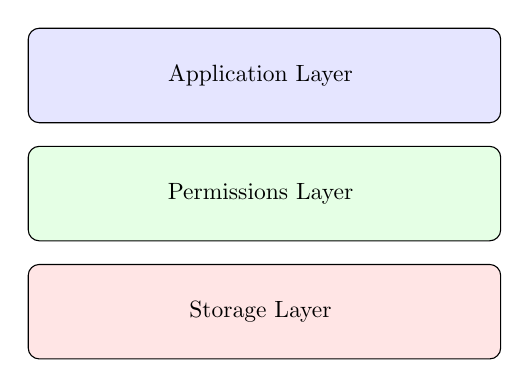
\begin{tikzpicture}[scale = 0.6, every node/.style={scale = 0.85}, every node/.append style={fill = white, rounded corners = 2pt, inner sep = 2pt, align = center}]
  
  % Layer boxes
  \draw [rounded corners, fill=blue!10] (-5, 3.5) rectangle (5, 1.5);
  \node [fill=blue!10] at (0, 2.5) { Application Layer };
  
  \draw [rounded corners, fill=green!10] (-5, 1) rectangle (5, -1);
  \node [fill=green!10] at (0, 0) { Permissions Layer };
  
  \draw [rounded corners, fill=red!10] (-5, -3.5) rectangle (5, -1.5);
  \node [fill=red!10] at (0, -2.5) { Storage Layer };
  
  \end{tikzpicture} \\
  \caption{
  	Platform Layers Overview
  }{
  	An overview of the layers of the platform from top to bottom. The permissions layer conceptually lies between the application layer and the storage layer, although in a decentralised system these layers act independently.
  }
  \label{fig:archi_platform_layers}
\end{figure}